\chapter{不變定律、四維向量與場張量}

我們先從一條自然界本可以遵守、實際上卻沒有遵守的定律談起。這條定律不成立，將告訴我們物理定律應如何書寫。同樣的檢驗，先讓我們從座標分量走向普通向量，再從普通向量走向四維向量，最後從四維向量走向張量。到最後，電場與磁場將不再是彼此分離的對象：它們會共同占據同一個反對稱張量中的六個獨立分量。

除非另有說明，我們採用\(c=1\)單位制，時空分量依\((1,2,3,0)=(x,y,z,t)\)排序，並使用度規號差\((-,-,-,+)\)。

\section{對稱性不正確的一種可能定律}

在空間中永久固定一條\(x\)軸和一條\(y\)軸。現在規定，只要兩個粒子的\(x\)座標相同，它們就會發生相互作用。這種相互作用可能使它們的運動反向，也可能使它們朝新的方向運動；具體的動力學並不重要。提出的觸發條件只有：
\begin{equation}
  x_1-x_2=0,
\end{equation}
其中下標標記的是粒子，而非座標分量。這條規則在數學上並無矛盾。問題是，為什麼它在物理上不太可信。

\begin{classroomqa}
\audiencequestion{這條規則違反空間的均勻性嗎？}
\lecturerresponse{不會。平移原點會使兩個座標增加相同的量，因此\(x_1-x_2\)保持不變。這條規則沒有指定任何優先位置。它的缺陷在於各向同性：它選定了一個優先方向。}
\end{classroomqa}

將座標軸旋轉\(90^\circ\)。原來的\(x\)方向現在稱為\(y\)，因此同一組物理事件會以\(y\)座標相等來描述。若旋轉角度一般，條件就會涉及\(x\)與\(y\)的線性組合。因此，定律的形式取決於黑板的擺放方向。它具有平移不變性，卻不具有旋轉不變性。

我們通常選用正交座標，使物理定律的形式最簡。也可以使用更一般的座標，但度規和公式就會比較複雜。在正交笛卡兒座標系中，不應有任何一種取向特別受到偏好。

修正方式很直接。在二維空間中，要求兩個座標都相同；在三維空間中，則要求三個座標都相同：
\begin{equation}
  x_1=x_2,
  \qquad y_1=y_2,
  \qquad z_1=z_2.
\end{equation}
如此一來，粒子只有在抵達同一點時才會相互作用，即使它們是沿著不同直線接近該點。

\begin{classroomqa}
\audiencequestion{\(z\)座標和時間也必須相同嗎？}
\lecturerresponse{在三維空間中，\(z\)座標也必須相同。這裡暫且略去時間；空間上的論證一完成，就會把時間納入。}
\end{classroomqa}

設\(\boldsymbol r_a\)為粒子\(a\)的位置。三個分量條件可以合寫成一個向量方程：
\begin{equation}
  \boldsymbol r_1-\boldsymbol r_2=\boldsymbol 0.
\end{equation}
某個分量在一個旋轉後的座標系中可能為零，在另一個座標系中卻不為零。整個向量則不同：若它在一個座標系中的每個分量都為零，那麼在任何旋轉後的座標系中，每個分量也都為零。同樣地，若兩個向量在一個座標系中相等，對兩者施行變換後，它們仍然相等。

\begin{figure}[H]
\centering
\includegraphics[width=0.78\textwidth]{lecture_06_figure_01.png}
\caption{這三個座標等式確保碰撞代表空間位置重合，而不是只在某個優先軸上座標相同。}
\lectureframe{00:09:00}
\end{figure}

這就是向量方程有用的原因。向量的分量會改變，但整個對象的變換方式彼此一致。以完整向量表示的定律，在旋轉座標時可以維持原有形式。

\section{時空中的重合}

現在把垂直的空間軸換成時間。一條牛頓式的規則可能會說，兩次運動變化只有在同一時間發生時才會發生。在牛頓力學中，所有慣性觀察者對同時性的判定一致，因此這樣的規則是可行的。但在狹義相對論中，這條規則會選出一個優先參考系。在一個參考系中同時發生的事件，在另一個參考系中未必同時。

只要求空間座標相同也不夠。一個時空位移的空間分量可以全為零，但時間分量不為零：
\begin{equation}
  \Delta X^\mu=(0,0,0,\Delta t),
\end{equation}
而洛倫茲推進會將\(\Delta t\)與空間分量混合。不變的局域陳述是，兩次運動變化發生在同一個事件。因此，簡單的碰撞要求：
\begin{equation}
  X_1^\mu=X_2^\mu,
  \qquad\text{or}\qquad
  X_1^\mu-X_2^\mu=0.
\end{equation}
四個座標都相同：粒子在同一時間位於同一地點。

碰撞的例子引出一條書寫物理定律的一般原則：可以把所有項移到等式的一側，令完整的四維向量等於零；也可以令一個完整的四維向量等於另一個。只把四維向量中彼此分離的分量拿來相等，本身並不能構成洛倫茲不變的陳述。

\section{洛倫茲推進、旋轉與矩陣記法}

四維向量是一種依照時空位移的方式變換的對象。要讓這個定義便於使用，先回顧座標本身如何變換。對於沿\(x\)方向、速度為\(v\)的洛倫茲推進，
\begin{align}
  x'&=\gamma(x-vt), & y'&=y, & z'&=z,
  & t'&=\gamma(t-vx),                                      \label{eq:l6-boost}
\end{align}
其中
\begin{equation}
  \gamma(v)=\frac{1}{\sqrt{1-v^2}}.
\end{equation}

\begin{classroomqa}
\audiencequestion{這些公式中是否已把光速設為 1？}
\lecturerresponse{是。恢復單位後，令\(X^0=ct\)，將\(1-v^2\)換成\(1-v^2/c^2\)，並在混合的空間--時間項中補回相應的\(c\)因子。}
\end{classroomqa}

繞\(z\)軸旋轉時，\(x\)和\(y\)會彼此混合，而\(z\)和\(t\)保持不變：
\begin{equation}
\begin{pmatrix}
  x'\\ y'\\ z'\\ t'
\end{pmatrix}
=
\begin{pmatrix}
  \cos\theta & \sin\theta & 0 & 0\\
  -\sin\theta & \cos\theta & 0 & 0\\
  0 & 0 & 1 & 0\\
  0 & 0 & 0 & 1
\end{pmatrix}
\begin{pmatrix}
  x\\ y\\ z\\ t
\end{pmatrix}.
\end{equation}
值得把零也寫出來，因為它們清楚顯示哪些分量不會影響某個變換後的座標。依照相同的分量順序，式~\eqref{eq:l6-boost}中的洛倫茲推進為
\begin{equation}
\begin{pmatrix}
  x'\\ y'\\ z'\\ t'
\end{pmatrix}
=
\begin{pmatrix}
  \gamma & 0 & 0 & -\gamma v\\
  0 & 1 & 0 & 0\\
  0 & 0 & 1 & 0\\
  -\gamma v & 0 & 0 & \gamma
\end{pmatrix}
\begin{pmatrix}
  x\\ y\\ z\\ t
\end{pmatrix}.
\end{equation}

旋轉與洛倫茲推進可以用矩陣乘法複合。若要沿著與原本\(x\)軸不對齊的方向推進，可以先旋轉座標，使該方向對準\(x\)軸，再施行推進，之後視需要旋轉座標。這些基本矩陣的乘積可以構成更一般的洛倫茲變換。

\begin{classroomqa}
\audiencequestion{先旋轉再推進，和先推進再旋轉，有差別嗎？}
\lecturerresponse{有。第一次操作之後，第二次操作所依據的軸已經改變。兩種矩陣乘積不一定相同，因此操作順序有影響。}
\end{classroomqa}

所有這些線性變換都可以統一寫成
\begin{equation}
  X'^{\mu}=\Lambda^{\mu}{}_{\nu}X^{\nu}.                  \label{eq:l6-vector-transform}
\end{equation}
重複指標\(\nu\)表示對\(1,2,3,0\)求和。這只是用指標記法表示矩陣乘法中通常的逐列逐行求和。

\begin{figure}[H]
\centering
\includegraphics[width=0.78\textwidth]{lecture_06_figure_02.png}
\caption{上方的指標形式洛倫茲變換，以及其欄向量形式的開頭。}
\lectureframe{00:31:55}
\end{figure}

式~\eqref{eq:l6-vector-transform}也定義了一般的逆變四維向量。若\(A^\mu\)是這樣的向量，則
\begin{equation}
  A'^{\mu}=\Lambda^{\mu}{}_{\nu}A^{\nu}.
\end{equation}
它的四個分量不一定代表位置。使這個對象成為四維向量的，是它的變換定律。

\section{標量、度規與不變內積}

在使用更多四維向量之前，先回頭看看較簡單的標量概念會有所幫助。在空間旋轉下，某一指定位置的溫度是標量，兩個指定位置之間的距離也是標量。兩者各是一個數，與座標軸的取向無關。甚至可以故意提出一個荒謬的數值主張：以公分量得的距離等於以華氏度量得的室溫。這個主張沒有什麼物理意義，但由於等式兩側都是旋轉標量，其真假不會因座標軸轉動而改變。

向量分量不是標量，因此我們需要一套有系統的方法，把它們組合成標量。將一般的逆變四維向量寫成
\begin{equation}
  A^\mu=(A^1,A^2,A^3,A^0).
\end{equation}
協變分量以較低的指標描述同一個幾何對象。在我們採用的號差下，它們由閔可夫斯基度規給出：
\begin{equation}
  A_\mu=\eta_{\mu\nu}A^\nu,
  \qquad
  \eta_{\mu\nu}=
  \begin{pmatrix}
    -1&0&0&0\\
    0&-1&0&0\\
    0&0&-1&0\\
    0&0&0&1
  \end{pmatrix},                                          \label{eq:l6-metric}
\end{equation}
因此
\begin{equation}
  A_\mu=(-A^1,-A^2,-A^3,A^0).
\end{equation}

\begin{classroomqa}
\audiencequestion{黑板上的兩個指標和正負號是否不一致？}
\lecturerresponse{是。所示欄向量中的空間分量應帶有相應的負號；指標降階方程右側的分量，在乘上\(\eta_{\mu\nu}\)之前也應帶有上標。時間標記是\(0\)，不是\(4\)。}
\end{classroomqa}

\begin{figure}[H]
\centering
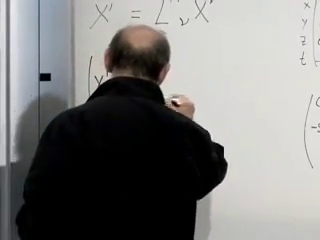
\includegraphics[width=0.8\textwidth]{lecture_06_figure_03.png}
\caption{逆變與協變分量、度規矩陣，以及不變縮併的開頭。}
\lectureframe{00:45:00}
\end{figure}

降指標並非只是裝飾。它把洛倫茲不變範數所需的正負號收納起來：
\begin{align}
  A_\mu A^\mu
  &=-(A^1)^2-(A^2)^2-(A^3)^2+(A^0)^2,                    \label{eq:l6-norm}\\
  X_\mu X^\mu
  &=t^2-x^2-y^2-z^2.
\end{align}
第二個式子是從原點到該事件的不變時空間隔。由於\(A^\mu\)和\(X^\mu\)的變換方式相同，它們的縮併也具有相同的不變性。

這種記法也帶出一條實用的記帳規則：重複的求和指標，一次寫在上方、一次寫在下方。例如：
\begin{equation}
  A_\mu A^\mu
  =\eta_{\mu\nu}A^\mu A^\nu.
\end{equation}
求和指標又稱啞指標，其名稱可以更改，而不影響所代表的量。

\begin{classroomqa}
\audiencequestion{其中一個向量是否應視為行向量，另一個視為列向量？它們的順序有影響嗎？}
\lecturerresponse{就目前的計算而言，把帶指標的量視為分量，並讓度規完成縮併即可；不必把討論轉成行與列的算符代數。這些量都是普通數，因此順序不影響結果。非對易算符則需要更仔細處理，但這不是此處討論的主題。}
\end{classroomqa}

同樣的構造也能定義兩個不同四維向量的內積：
\begin{equation}
  A\mathbin{\cdot}B=A_\mu B^\mu=A^\mu B_\mu.
\end{equation}
不必寫出明確的洛倫茲矩陣，就能看出它的不變性。由於\(A+B\)和\(A-B\)都是四維向量，它們的範數平方都是不變量：
\begin{align}
  (A+B)^2&=A^2+B^2+2A\mathbin{\cdot}B,\\
  (A-B)^2&=A^2+B^2-2A\mathbin{\cdot}B.
\end{align}
兩式相減可得
\begin{equation}
  (A+B)^2-(A-B)^2=4A\mathbin{\cdot}B,                    \label{eq:l6-polarization}
\end{equation}
因此\(A\mathbin{\cdot}B\)也是不變量。展開後即可直接得到因子 4。\editorialnote{黑板上的論證給出了這個極化恆等式；寫出因子 4，可以清楚交代口頭推導中的消去過程。}

\begin{figure}[H]
\centering
\includegraphics[width=0.8\textwidth]{lecture_06_figure_04.png}
\caption{用來分離不同四維向量內積的兩個不變平方。}
\lectureframe{00:52:20}
\end{figure}

不變量是構成物理定律的自然要素：不同於單獨的分量，它們在不同參考系中具有相同的值。

\section{固有速度與四維動量}

考慮粒子世界線上兩個相鄰的事件。它們之間的間隔是無窮小四維向量：
\begin{equation}
  dX^\mu=(dx,dy,dz,dt).
\end{equation}
對於類時世界線，固有時間定義為
\begin{equation}
  d\tau^2=dX_\mu dX^\mu
  =dt^2-dx^2-dy^2-dz^2.                                  \label{eq:l6-proper-time}
\end{equation}
固有四維速度為
\begin{equation}
  U^\mu=\frac{dX^\mu}{d\tau}.                            \label{eq:l6-four-velocity}
\end{equation}
它衡量時空位置相對於粒子自身固有時間的變化率，而不是相對於某個選定參考系的座標時間。

雖然\(U^\mu\)有四個分量，但只有三個彼此獨立。將式~\eqref{eq:l6-proper-time}除以\(d\tau^2\)可得
\begin{equation}
  U_\mu U^\mu=1.
\end{equation}
因此，四維速度是單位類時向量。選擇指向未來的方向，就確定了它的時間分量符號。

\begin{classroomqa}
\audiencequestion{當速度遠小於\(c\)時，四維速度會趨近普通速度嗎？}
\lecturerresponse{它的三個空間分量會趨近普通速度，而時間分量在\(c=1\)單位制下趨近於 1。這個關係可由鏈鎖律並計算\(dt/d\tau\)得到。}
\end{classroomqa}

對每個空間分量，
\begin{equation}
  U^i=\frac{dx^i}{d\tau}
     =\frac{dx^i}{dt}\frac{dt}{d\tau}
     =v^i\frac{dt}{d\tau}.
\end{equation}
將式~\eqref{eq:l6-proper-time}除以\(dt^2\)：
\begin{equation}
  \left(\frac{d\tau}{dt}\right)^2
  =1-v_x^2-v_y^2-v_z^2
  =1-\boldsymbol v^2.
\end{equation}
因此
\begin{equation}
  \frac{dt}{d\tau}=\frac{1}{\sqrt{1-\boldsymbol v^2}}
  =\gamma(\lvert\boldsymbol v\rvert),
\end{equation}
並且
\begin{equation}
  U^\mu=(\gamma v_x,\gamma v_y,\gamma v_z,\gamma).
                                                                  \label{eq:l6-u-components}
\end{equation}

\begin{figure}[H]
\centering
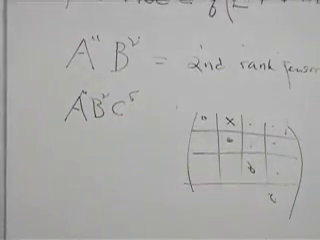
\includegraphics[width=0.8\textwidth]{lecture_06_figure_05.png}
\caption{透過固有時間計算得到\(dt/d\tau=\gamma\)，並建立固有速度與普通速度之間的關係。}
\lectureframe{01:02:00}
\end{figure}

\begin{classroomqa}
\audiencequestion{\(dx^2/dt^2\)是指二階導數嗎？向量平方是否應該產生交叉項？}
\lecturerresponse{這裡指的是\((dx/dt)^2\)，也就是一階導數的平方。此外，\(\boldsymbol v^2\)表示歐幾里得內積\(v_x^2+v_y^2+v_z^2\)，而不是形式上的和\(v_x+v_y+v_z\)的平方，所以不會有交叉項。}
\end{classroomqa}

\begin{classroomqa}
\audiencequestion{\(\gamma(v)\)中的\(v\)，是兩個座標參考系之間的相對速度，還是粒子的速度？}
\lecturerresponse{這裡指粒子在所選參考系中的速度。函數\(\gamma(v)=1/\sqrt{1-v^2}\)可以用於任意速度：在洛倫茲推進中，代入的是參考系間的相對速度；在四維速度中，代入的則是粒子速度。}
\end{classroomqa}

當\(v\ll1\)時，\(\gamma\simeq1\)，因此\(U^\mu\)的空間分量會趨近\(\boldsymbol v\)，而\(U^0\)會趨近於 1。普通速度趨近光速時，\(\gamma\)會無界增大，四維速度所有非零分量也都會無界增大。

\begin{classroomqa}
\audiencequestion{\(U^0\)的量綱不是應該是速度嗎？為什麼它會接近數值 1？}
\lecturerresponse{把\(c\)設為 1 時，量綱就被省略了。若採用\(X^0=ct\)，則
\(U^\mu=(\gamma\boldsymbol v,\gamma c)\)，所以時間分量會趨近\(c\)，而且\(U_\mu U^\mu=c^2\)。}
\end{classroomqa}

對靜止質量為\(m\)的粒子，四維動量定義為
\begin{equation}
  P^\mu=mU^\mu.
\end{equation}
在自然單位制下，
\begin{equation}
  P^\mu=(\gamma m\boldsymbol v,\gamma m).
\end{equation}
低速時，前三個分量會趨近牛頓力學中的動量\(m\boldsymbol v\)。恢復單位後可得
\begin{equation}
  P^\mu=(\gamma m\boldsymbol v,E/c),
  \qquad E=\gamma mc^2,
\end{equation}
因此
\begin{equation}
  E=mc^2+\frac{1}{2}m\boldsymbol v^2+O(mv^4/c^2).
\end{equation}
時間分量以\(c=1\)為單位表示能量；若四個分量都以動量為單位，則時間分量是能量除以\(c\)。

\begin{classroomqa}
\audiencequestion{在普通\(\boldsymbol v\)後面加上一個第四分量，所得的量本身是四維向量嗎？}
\lecturerresponse{不是。普通三維速度的變換方式並非四維向量的變換方式。因子\(\gamma\)和固有時間的定義不可或缺；四維向量是\(U^\mu\)，不是\(\boldsymbol v\)。}
\end{classroomqa}

\section{為何電場與磁場必須彼此混合}

現在我們暫時離開相對論一下。從愛因斯坦之前的運動方程出發，看看要讓它適用於所有慣性參考系，必須如何重新整理。普通加速度是普通速度對時間的導數。它在四維時空中的對應量自然是
\begin{equation}
  A^\mu=\frac{dU^\mu}{d\tau}.
\end{equation}
低速時，它的空間分量會趨近普通加速度。完整的相對論方程稍後再談；我們先看看舊的力定律。

電荷\(q\)處於電場和磁場中時，
\begin{equation}
  \boldsymbol F=m\boldsymbol a
  =q\left(\boldsymbol E+\boldsymbol v\times\boldsymbol B\right).
                                                                  \label{eq:l6-lorentz-force}
\end{equation}
電場項與粒子速度無關，磁場項則與粒子速度有關。

\begin{figure}[H]
\centering
\includegraphics[width=0.8\textwidth]{lecture_06_figure_06.png}
\caption{促使我們將\(\boldsymbol E\)與\(\boldsymbol B\)合併考慮的前相對論洛倫茲力定律。}
\lectureframe{01:18:20}
\end{figure}

假設某位觀察者看不到電場，卻看到磁場和一個運動中的電荷。電荷會受到磁力。然而，在電荷的瞬時靜止參考系中，\(\boldsymbol v=0\)，因此式~\eqref{eq:l6-lorentz-force}中的磁場項便消失。座標改變不會使實際的世界線變成慣性運動；因此新參考系中的力必須包含電場的貢獻。更精確地說，非零的四維加速度不可能只靠轉換慣性參考系就變為零，即使三維加速度及其分量確實會隨參考系而變。\editorialnote{四維加速度的這項陳述是不變的課堂論證形式，也避免把普通三維加速度本身誤當成參考系不變量。}

因此，電場和磁場必須彼此轉換。兩者合計有六個分量，所以它們既不是單一標量，也不是單一四維向量。我們需要一種新的變換對象。

\section{張量：每個指標各對應一次變換}

標量可視為零階張量，沒有指標。四維向量是階數為一的張量，帶有一個可取四種值的指標。最簡單的二階例子是兩個向量的乘積：
\begin{equation}
  A^\mu B^\nu.
\end{equation}
每個指標有四種可能，因此這個對象有\(4^2=16\)個分量，可以排成\(4\times4\)陣列。三個向量的乘積
\begin{equation}
  A^\mu B^\nu C^\sigma,
\end{equation}
有\(4^3=64\)個分量，是三階張量。更高階張量也依此類推。名稱不如定義對象的規則重要。

若
\begin{equation}
  A'^{\mu}=\Lambda^\mu{}_{\nu}A^\nu,
  \qquad
  B'^{\sigma}=\Lambda^\sigma{}_{\tau}B^\tau,
\end{equation}
則兩者的乘積會按下式變換：
\begin{equation}
  A'^{\mu}B'^{\sigma}
  =\Lambda^\mu{}_{\nu}\Lambda^\sigma{}_{\tau}
   A^\nu B^\tau.
\end{equation}
這就是逆變二階張量的定義變換律：
\begin{equation}
  T'^{\mu\sigma}
  =\Lambda^\mu{}_{\nu}\Lambda^\sigma{}_{\tau}T^{\nu\tau}.
                                                                  \label{eq:l6-tensor-transform}
\end{equation}
每個指標各對應一個洛倫茲矩陣。重複的\(\nu\)和\(\tau\)要對其求和；未縮併的\(\mu\)和\(\sigma\)則標示在帶撇參考系中所求的分量。

\begin{figure}[H]
\centering
\includegraphics[width=0.82\textwidth]{lecture_06_figure_07.png}
\caption{兩個向量的變換方式，以及由此得到的二階張量雙矩陣變換律。}
\lectureframe{01:27:15}
\end{figure}

張量不一定是單一的向量乘積。\(A^\mu B^\nu\)和\(A^\nu B^\mu\)都遵守張量變換律，它們的和，以及像下式這樣的和也一樣：
\begin{equation}
  A^\mu B^\nu+C^\mu D^\nu.
\end{equation}
張量的定義是其變換律，而非某種特定的因式分解。三階張量會多出第三個洛倫茲矩陣，依此類推。

\section{對稱張量與反對稱張量}

有兩類二階張量特別有用。對稱張量滿足
\begin{equation}
  T^{\mu\nu}=T^{\nu\mu},
\end{equation}
也就是說，對角線兩側互為鏡像的矩陣元相等。四個對角矩陣元，加上對角線一側的六個矩陣元，即可決定其餘部分，因此共有
\begin{equation}
  4+6=10
\end{equation}
個獨立分量。

反對稱張量滿足
\begin{equation}
  T^{\mu\nu}=-T^{\nu\mu}.                                \label{eq:l6-antisymmetry}
\end{equation}
在式~\eqref{eq:l6-antisymmetry}中令\(\mu=\nu\)，可得
\(T^{\mu\mu}=-T^{\mu\mu}\)，因此所有對角矩陣元都為零。三角形一側的六個矩陣元，決定另一側對應的六個矩陣元，符號則相反。因此恰有六個獨立分量。

\begin{figure}[H]
\centering
\includegraphics[width=0.82\textwidth]{lecture_06_figure_08.png}
\caption{完整的反對稱\(4\times4\)陣列：對角線上的元素為零，對角線兩側的元素符號相反。}
\lectureframe{01:34:25}
\end{figure}

這個數目正是線索。三個電場分量和三個磁場分量，恰好可以放進一個反對稱二階張量。

\section{電磁場張量}

令時空指標依照\((1,2,3,0)=(x,y,z,t)\)的順序排列在各列與各行。黑板上的排列方式是
\begin{equation}
  F_{\mu\nu}=
  \begin{pmatrix}
    0    & -B_3 & B_2  & E_1\\
    B_3  & 0    & -B_1 & E_2\\
    -B_2 & B_1  & 0    & E_3\\
    -E_1 & -E_2 & -E_3 & 0
  \end{pmatrix}.                                         \label{eq:l6-field-tensor}
\end{equation}
純空間部分的矩陣元包含磁場；一個空間指標搭配一個時間指標的矩陣元則包含電場。知道上三角部分後，便可由反對稱性得出下三角部分。

\begin{classroomqa}
\audiencequestion{磁場的矩陣元是否全為負號？這些指標是否對應於\(x,y,z\)？}
\lecturerresponse{上三角空間部分的符號交替如下：\(-B_3,+B_2,-B_1\)。指標\(1,2,3\)對應於\(x,y,z\)，而\(0\)代表時間。沿對角線反射時，每個符號都會反轉。}
\end{classroomqa}

\begin{figure}[H]
\centering
\includegraphics[width=0.82\textwidth]{lecture_06_figure_09.png}
\caption{依照這堂課中空間分量優先的順序排列的完整電磁場張量。}
\lectureframe{01:41:05}
\end{figure}

慣例上，這個張量記為\(F_{\mu\nu}\)，而非一般的\(T_{\mu\nu}\)。講師猜測這個字母可能代表法拉第，但也明確表示自己不知道這個記號的歷史。此處重要的是它的反對稱性和六個場分量，而不是對字母來源的猜測。

\begin{classroomqa}
\audiencequestion{矩陣中的每個元素，是否代表該座標平面上的場強？}
\lecturerresponse{每個元素都是電磁場張量的一個分量。含有時間指標的元素代表電場分量，而空間--空間元素則編碼磁場分量。}
\end{classroomqa}

將含時間指標的那一列和那一行分隔出來。剩下的\(3\times3\)反對稱區塊代表磁場。它的獨立分量可以用循環方式記憶：
\begin{equation}
  F_{12}=-B_3,
  \qquad F_{23}=-B_1,
  \qquad F_{31}=-B_2.                                   \label{eq:l6-magnetic-cycle}
\end{equation}
從第一個關係式開始，讓各指標依\(1\to2\to3\to1\)的順序循環。等價地，
\begin{equation}
  F_{ij}=-\epsilon_{ijk}B_k,
\end{equation}
其中\(\epsilon_{123}=+1\)。\editorialnote{Levi--Civita 公式是循環規則的標準簡潔寫法；這條規則已在黑板上逐項推導。}

\begin{figure}[H]
\centering
\includegraphics[width=0.82\textwidth]{lecture_06_figure_10.png}
\caption{反對稱張量中編碼磁場的循環空間分量。}
\lectureframe{01:46:20}
\end{figure}

電場的對應關係更直接：
\begin{equation}
  E_1=F_{10},
  \qquad E_2=F_{20},
  \qquad E_3=F_{30}.
\end{equation}

因此，磁場有兩種有用的表示方式。在三維空間中，三分量的軸向量可以和一個\(3\times3\)反對稱張量相互對應。然而在時空中，磁場只是六分量張量\(F_{\mu\nu}\)的空間部分。這種對應方式是三維空間所特有的：一個反對稱的\(4\times4\)張量有六個獨立分量，無法等同於四維向量。\editorialnote{在正旋轉下，磁場的變換方式如同向量；在反射下，更精確地說，它是軸向量，也就是偽向量。}

這項建構的目的並非只為了計算分量數目。由於\(F_{\mu\nu}\)依張量的方式變換，洛倫茲推進會自動混合其中的電場分量與磁場分量。下一講會將它與四維速度和四維加速度結合，以協變運動方程取代式~\eqref{eq:l6-lorentz-force}。

\section{關於愛因斯坦與閔可夫斯基的問題}

最後幾分鐘的討論從形式體系轉向它的歷史起源。講者以回憶而非定論的方式回答；這項限定也是這段問答的一部分。

\begin{classroomqa}
\audiencequestion{愛因斯坦是基於概念上的理由尋求洛倫茲不變的表述，還是受到特定觀測結果的驅使？}
\lecturerresponse{自然定律在所有慣性參考系中都應具有相同形式，這項原理是他推理的核心。當時也有關於光的實驗證據，以及未能探測到相對於以太運動的結果；不過講師明確表示，他不確定愛因斯坦當時知道哪些結果，也不確定這些結果對他的影響有多大。概念上的要求是，麥克斯韋方程組與洛倫茲力都應遵守相對性原理，而這要求電場、磁場和速度分量一起變換。}
\end{classroomqa}

愛因斯坦在1905年的論述沒有使用此處採用的簡潔四維向量記法，而是逐一處理各分量，並明確寫出所需的\(\gamma\)因子和速度。之後，閔可夫斯基以幾何方式將同樣的結構整理成四維時空。

\begin{classroomqa}
\audiencequestion{愛因斯坦是否抗拒閔可夫斯基的時空表述？閔可夫斯基又是在多久之後提出這種表述？}
\lecturerresponse{課堂上講者的回憶是，愛因斯坦起初不太接受四維幾何的說法，但很快便認同它的價值。講者暫且估計，這大約是在1905年的論文之後兩年，也許是1907年；他強調自己是在回憶，而非確定歷史事實。}
\end{classroomqa}

\begin{classroomqa}
\audiencequestion{閔可夫斯基是數學家還是物理學家？他還有哪些貢獻？他是否受到洛倫茲或菲茨傑拉德的影響？}
\lecturerresponse{講者沒有聲稱自己能給出確定答案。數學家和物理學家的區別沒有進一步討論；一位聽眾提出更正，打斷了講者對閔可夫斯基其他工作的概略評論；至於可能的影響來源，講者也明確表示尚不確定。就這段討論而言，可以確定的是，閔可夫斯基以四維幾何記法，對相對論作了關鍵性的整理。}
\end{classroomqa}

\begin{classroomqa}
\audiencequestion{混合\(\boldsymbol E\)與\(\boldsymbol B\)的變換，在愛因斯坦1905年的工作中就已經出現了嗎？}
\lecturerresponse{有，但當時是逐一寫出各分量，而不是寫成單一的場張量方程。課堂上拿麥克斯韋的分量方程作比較：在能揭示共同結構的簡潔記法出現之前，相關內容就已經存在。閔可夫斯基的貢獻，是用時空語言有系統地呈現這個結構。}
\end{classroomqa}

這讓我們回到一開始提出的數學要點。分量對於計算不可或缺，但唯有將它們理解為同一個會變換的物件之組成部分，定律才變得清晰易懂。接下來要做的是利用\(F_{\mu\nu}\)，將帶電粒子的運動方程寫成在所有慣性系中形式皆相同的樣子。